\documentclass{article}
\usepackage[LGR,T1]{fontenc}
\usepackage[utf8]{inputenc}
\usepackage[greek, english]{babel}
\usepackage{alphabeta}
\usepackage{natbib}
\usepackage{graphicx}
\usepackage{biblatex}
\addbibresource{references.bib}

\def\code#1{\texttt{#1}}

\usepackage{eso-pic}% http://ctan.org/pkg/eso-pic
\usepackage{lipsum}% http://ctan.org/pkg/lipsum

\title{Robustness Diagrams - v0.2}

\author{\\

\includegraphics[width=3in]{safeguard}\\[1ex]\\\\
}

\begin{document}

\maketitle

\newpage

\noident Editor: Θεόδωρος Ντάκουρης - ntakouris@ceid.upatras.gr - 1054332\\
Contributor: Βάιος Λασκαρέλιας - laskarelias@ceid.upatras.gr - 1054432\\

\begin{tabular}{|l|c|c|}
\hline
Όνοματεπώνυμο & email & Αριθμός μητρώου  \\
\hline
Θεόδωρος Ντάκουρης & ntakouris@ceid.upatras.gr & 1054332 \\
Βασίλειος Βασιλόπουλος & vvasil@ceid.upatras.gr &  1054410 \\
Νικόλαος Σουλτάνης & soultanis@ceid.upatras.gr & 1054319  \\
Βάιος Λασκαρέλιας & laskarelias@ceid.upatras.gr & 1054432 \\
Αντόν Παπά & papa@ceid.upatras.gr & 1054337 \\
\hline
\end{tabular}

\renewcommand{\contentsname}{Περιεχόμενα}
\tableofcontents

\section{Αλλαγές}
\subsection{v0.2}
\begin{itemize}
    \item Έγινε μετονομασία στα ui boundary objects για να συμβαδίζουν με αυτά που θα δηλωθούν στο sequence, στο domain και στο κώδικα. Έχουν prefix "Ui\_"
    \item Άλλαξε η ροή του insert και delete user - employee ώστε να γίνεται πρώτα το pin authorization και μετά το προαιρετικό document save.
    \item Αφαιρέθηκε το Main Menu Notification boundary object, η λειτουργικότητά του συμπεριλαμβάνεται στο Main Menu.
    \item Αφαιρέθηκαν σε μερικά σημεία -Data suffixes για να υπάρχει naming consistency με το domain model
    \item Στο CheckIn - Out αφαιρέθηκε σε ένα σημεία αχρείαστη επικοινωνία controller με το RFID Card Scanner.
    \item Σε πολλά σημεία έγιναν μερικές renaming αλλαγές όταν διαπιστώνεται πως υπάρχει διπλή λειτουργικότητα ή πρέπει να γίνει σαφέστερο το όνομα (όπως για παράδειγμα, στο Incident Submission άλλαξε το 'Write to Access Logs' σε 'Write Incident to Access Logs') Αυτά τα πιο συγκεκριμένα ονόματα δεν αλλάζουν καθόλου τη σημασιολογία του εκάστοτε robustness διαγράμματος γιατί γίνεται αντιληπτή η ίδια ενέργεια με βάση τις γειτονικές ακμές του controller.
    \item Στα σημεία που υπήρχαν 2 συνδέσεις σε entity object από controller, προστέθηκε ένας ακόμα controller για να γίνει πιο καθαρή η διατύπωση.
    
    \hline
    \item Αφαιρέθηκαν - διορθώθηκαν όλα τα διπλότυπα boundary objects
    \item Διορθώθηκαν τα λάθος κυκλάκια που αντικατοπτρίζουν use case invocations (pin authorization, drone control)
    \item Διορθώθηκαν 2 σημεία παράνομης επικοινωνίας με βελάκι
    \item Απλοποιήθηκε η ροή του Search Access Logs, χωρίς επιρροή στην λειτουργικότητά του
    \hline
\end{itemize}

\section{Διαγράμματα}
Για δική σας ευκολία παρακαλώ να δείτε πέρα από τα screenshots το παρακάτω view-only link από draw.io:

\url{https://drive.google.com/file/d/1SifzHE3GUQTPN5xLYlfNoIiO4ZW4xI-G/view?usp=sharing}

\subsection{Check In-Out}

\noindent Σημείωση: Παρουσιάζονται και οι 2 περιπτώσεις "μαζί". Τις συγχωνεύουμε για λόγους επαναχρησιμοποίησης και ευαναγνωσίας-ευκολίας. Στην εναλλακτική περίπτωση, ο λόγος αποτυχίας - reason μεταβιβάζεται από controller σε controller μέχρι να φτάσει σε boundary object.

\noindent Check In-Out: \\
\noindent\makebox[\textwidth]{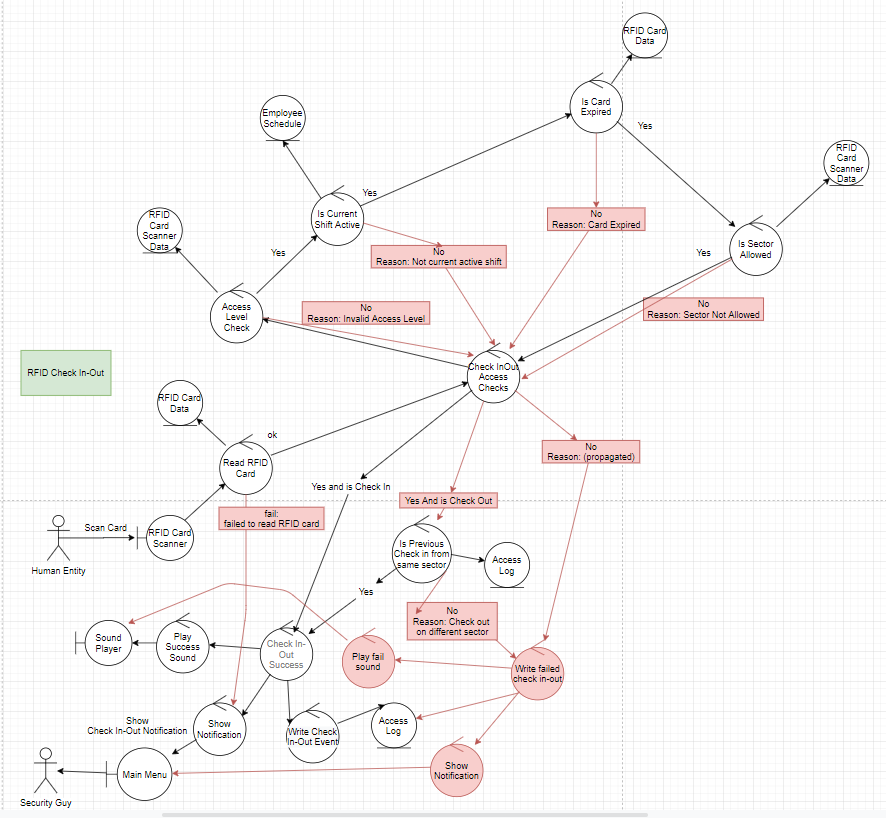
\includegraphics[width=\paperwidth]{rob-rfid.png}}

\subsection{Insert Employee}
\noindent\makebox[\textwidth]{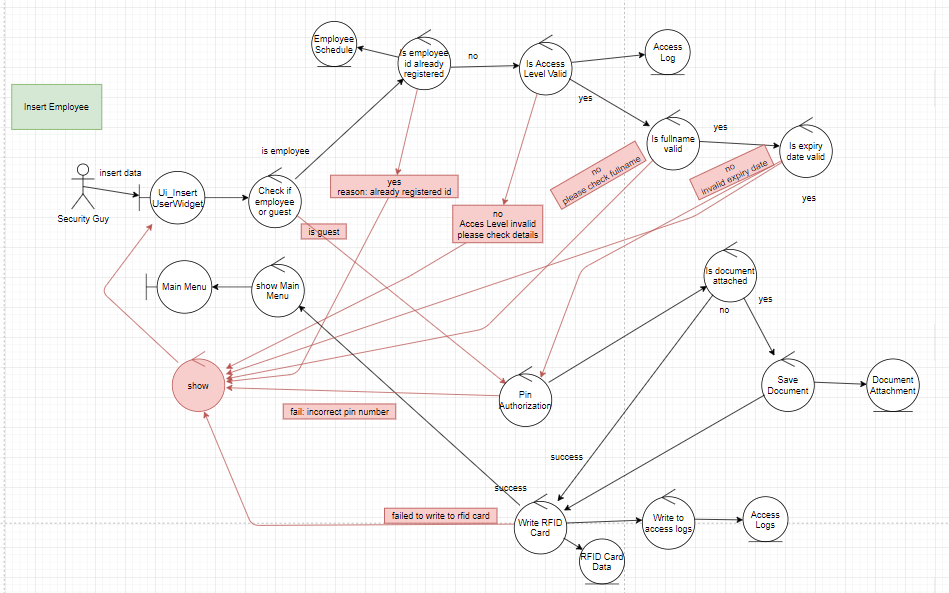
\includegraphics[width=\paperwidth]{rob-insert.png}}

\subsection{Delete Employee}
\noindent\makebox[\textwidth]{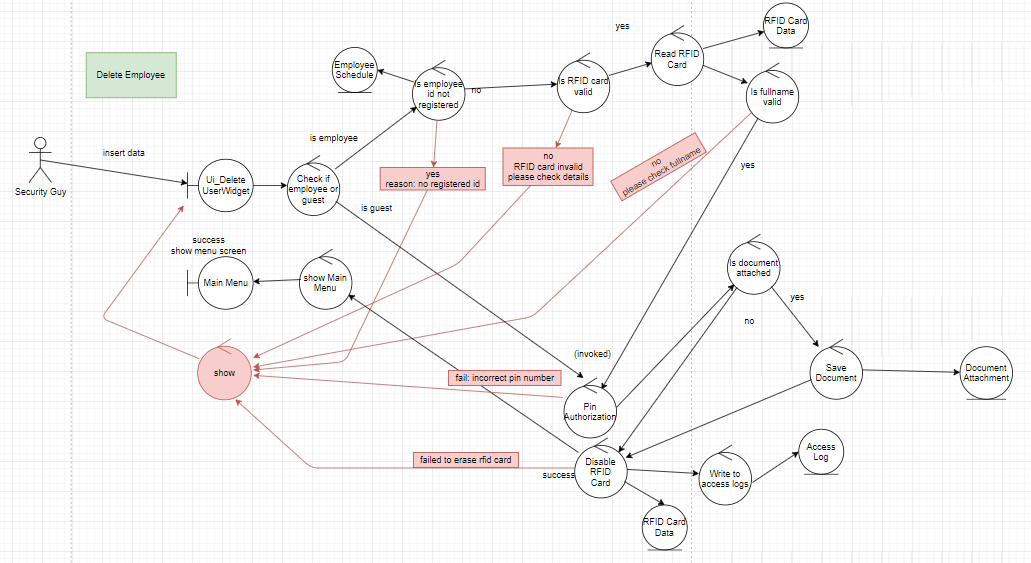
\includegraphics[width=\paperwidth]{rob-delete.png}}

\subsection{Search Access Logs}
\noindent\makebox[\textwidth]{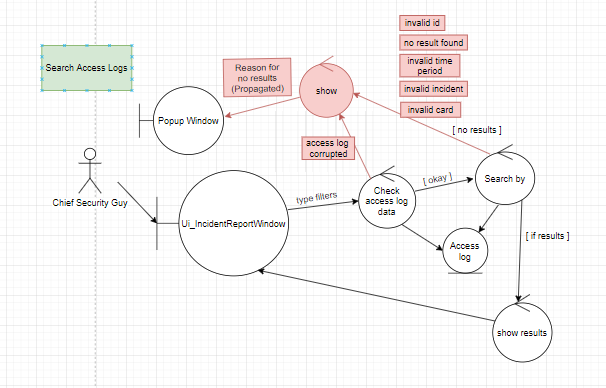
\includegraphics[width=\paperwidth]{rob-search.png}}

\subsection{Drone Notifications}
\noindent\makebox[\textwidth]{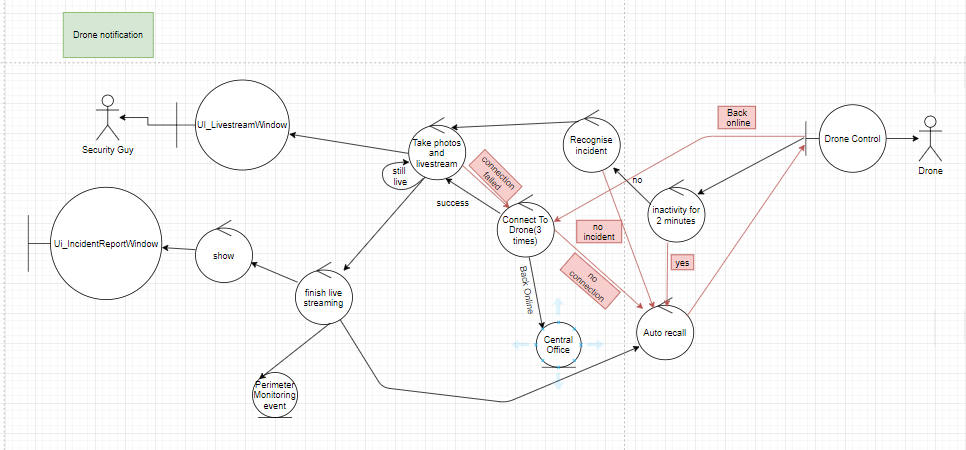
\includegraphics[width=\paperwidth]{rob-drone.png}}

\subsection{Incident Submission}
\noindent\makebox[\textwidth]{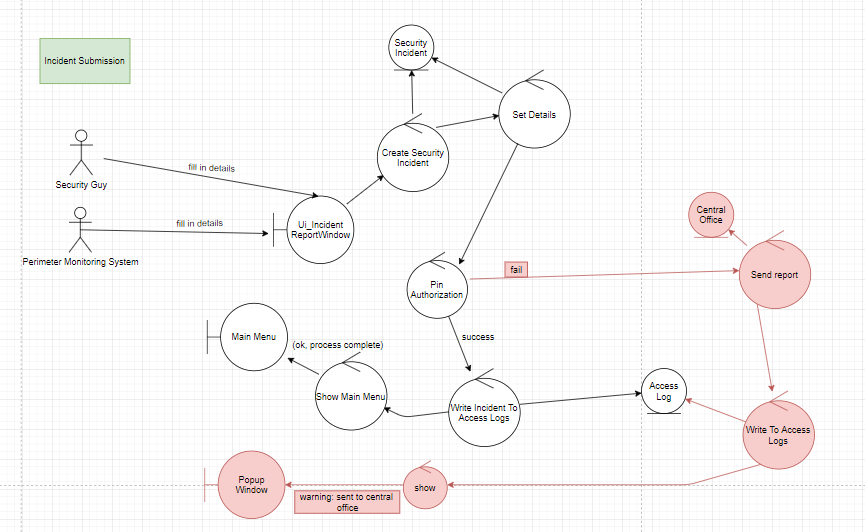
\includegraphics[width=\paperwidth]{rob-incident.png}}

\subsection{Send Drone}
\noindent\makebox[\textwidth]{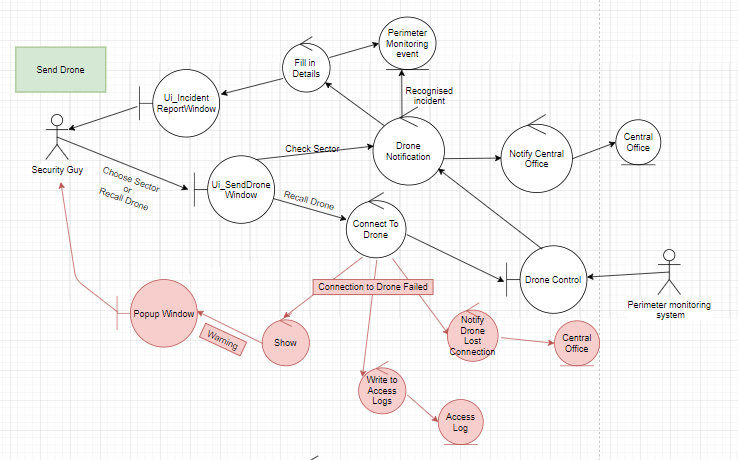
\includegraphics[width=\paperwidth]{rob-send.png}}

\subsection{Silent Alarm}
\noindent\makebox[\textwidth]{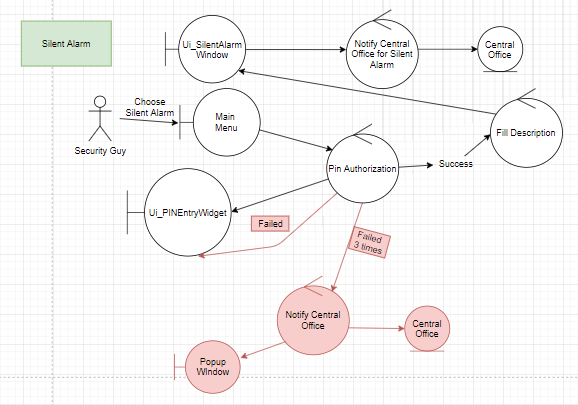
\includegraphics[width=\paperwidth]{rob-silent.png}}

\subsection{Pin Authorization}
\noindent\makebox[\textwidth]{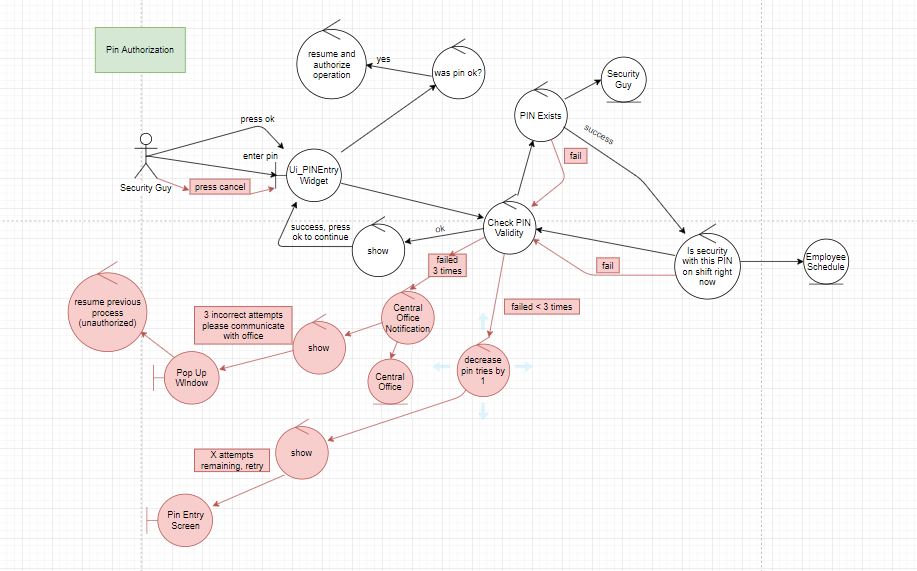
\includegraphics[width=\paperwidth]{rob-pin.png}}


\section{Εργαλεία}
Χρησιμοποιήθηκαν:
\begin{itemize}
    \item \LaTeX/Overleaf.com - Συγγραφή του παρόντος τεχνικού κειμένου
    \item Photoshop - Φωτογραφία Σελίδας Τίτλου
    \item draw.io - Σχεδιασμός διαγραμμάτων
\end{itemize}

\end{document}
